\chapter{Metodologia}

Este capítulo aborda o planejamento e execução do projeto, contendo os procedimentos e técnicas utilizadas, possibilitando a sua  replicação. Tendo em vista os conceitos descritos no capítulo \ref{cha:pln} (Processamento de Linguagem Natural), o presente trabalho tem como objetivo responder à seguinte questão problema:

\begin{center}
\textit{É possível extrair o perfil temático dos deputados através da análise dos seus discursos e proposições utilizando técnicas clássicas de aprendizado de máquina e processamento de linguagem natural?}
\end{center}

Além disso, será construído um \textit{web site} com o intuito de fornecer uma forma melhor de visualização dos dados obtidos nesta análise, através de gráficos interativos que garantam que o usuário tenha uma boa experiência de usabilidade.

\section{Trabalhos Relacionados}

Durante a pesquisa bibliográfica realizada neste trabalho, encontrou-se alguns trabalhos que também fizeram análise de textos parlamentares utilizando aprendizado Bayesiano. As seções a seguir descrevem brevemente alguns deles.

\subsection{Retórica Parlamentar}

O Retórica Parlamentar\footnote{http://retorica.labhackercd.net/about.html}, idealizado por Davi Moreira\footnote{https://github.com/davi-moreira}, Manoel Galdino\footnote{https://github.com/mgaldino} e Luís Carli\footnote{https://github.com/luiscarli}, utiliza os discursos proferidos pelos parlamentares no Pequeno Expediente e no Grande Expediente da Câmara dos Deputados para promover a transparência do mandato e fornecer subsídios para o controle social com a divulgação dos temas mais debatidos em Plenário.

A técnica utilizada pelo Retórica para a classificação dos discursos é um modelo Bayesiano hierárquico, descrito por \citeonline{grimmer2009}, onde através de aprendizado não supervisionado são gerados \(k\) \textit{clusters}, sendo \(k\) um valor escolhido ao executar o algoritmo. O resultado é exportado para o formato \textit{csv} e contém os termos mais frequentes de cada cluster. Em seguida, um especialista deve ler e rotular cada \textit{cluster}.

A visualização dos dados é feita através de um gráfico de bolhas, em que cada bolha representa a relevância (medida pela frequência) de cada tema dentre todos os deputados analisados. Dentro de cada bolha são colocados os deputados que enfatizam aquele tema nos seus discursos. Um deputado está associado a um único tema, que é o tema mais enfatizado por ele nos seus discursos.

\begin{figure}[h]
    \centering
    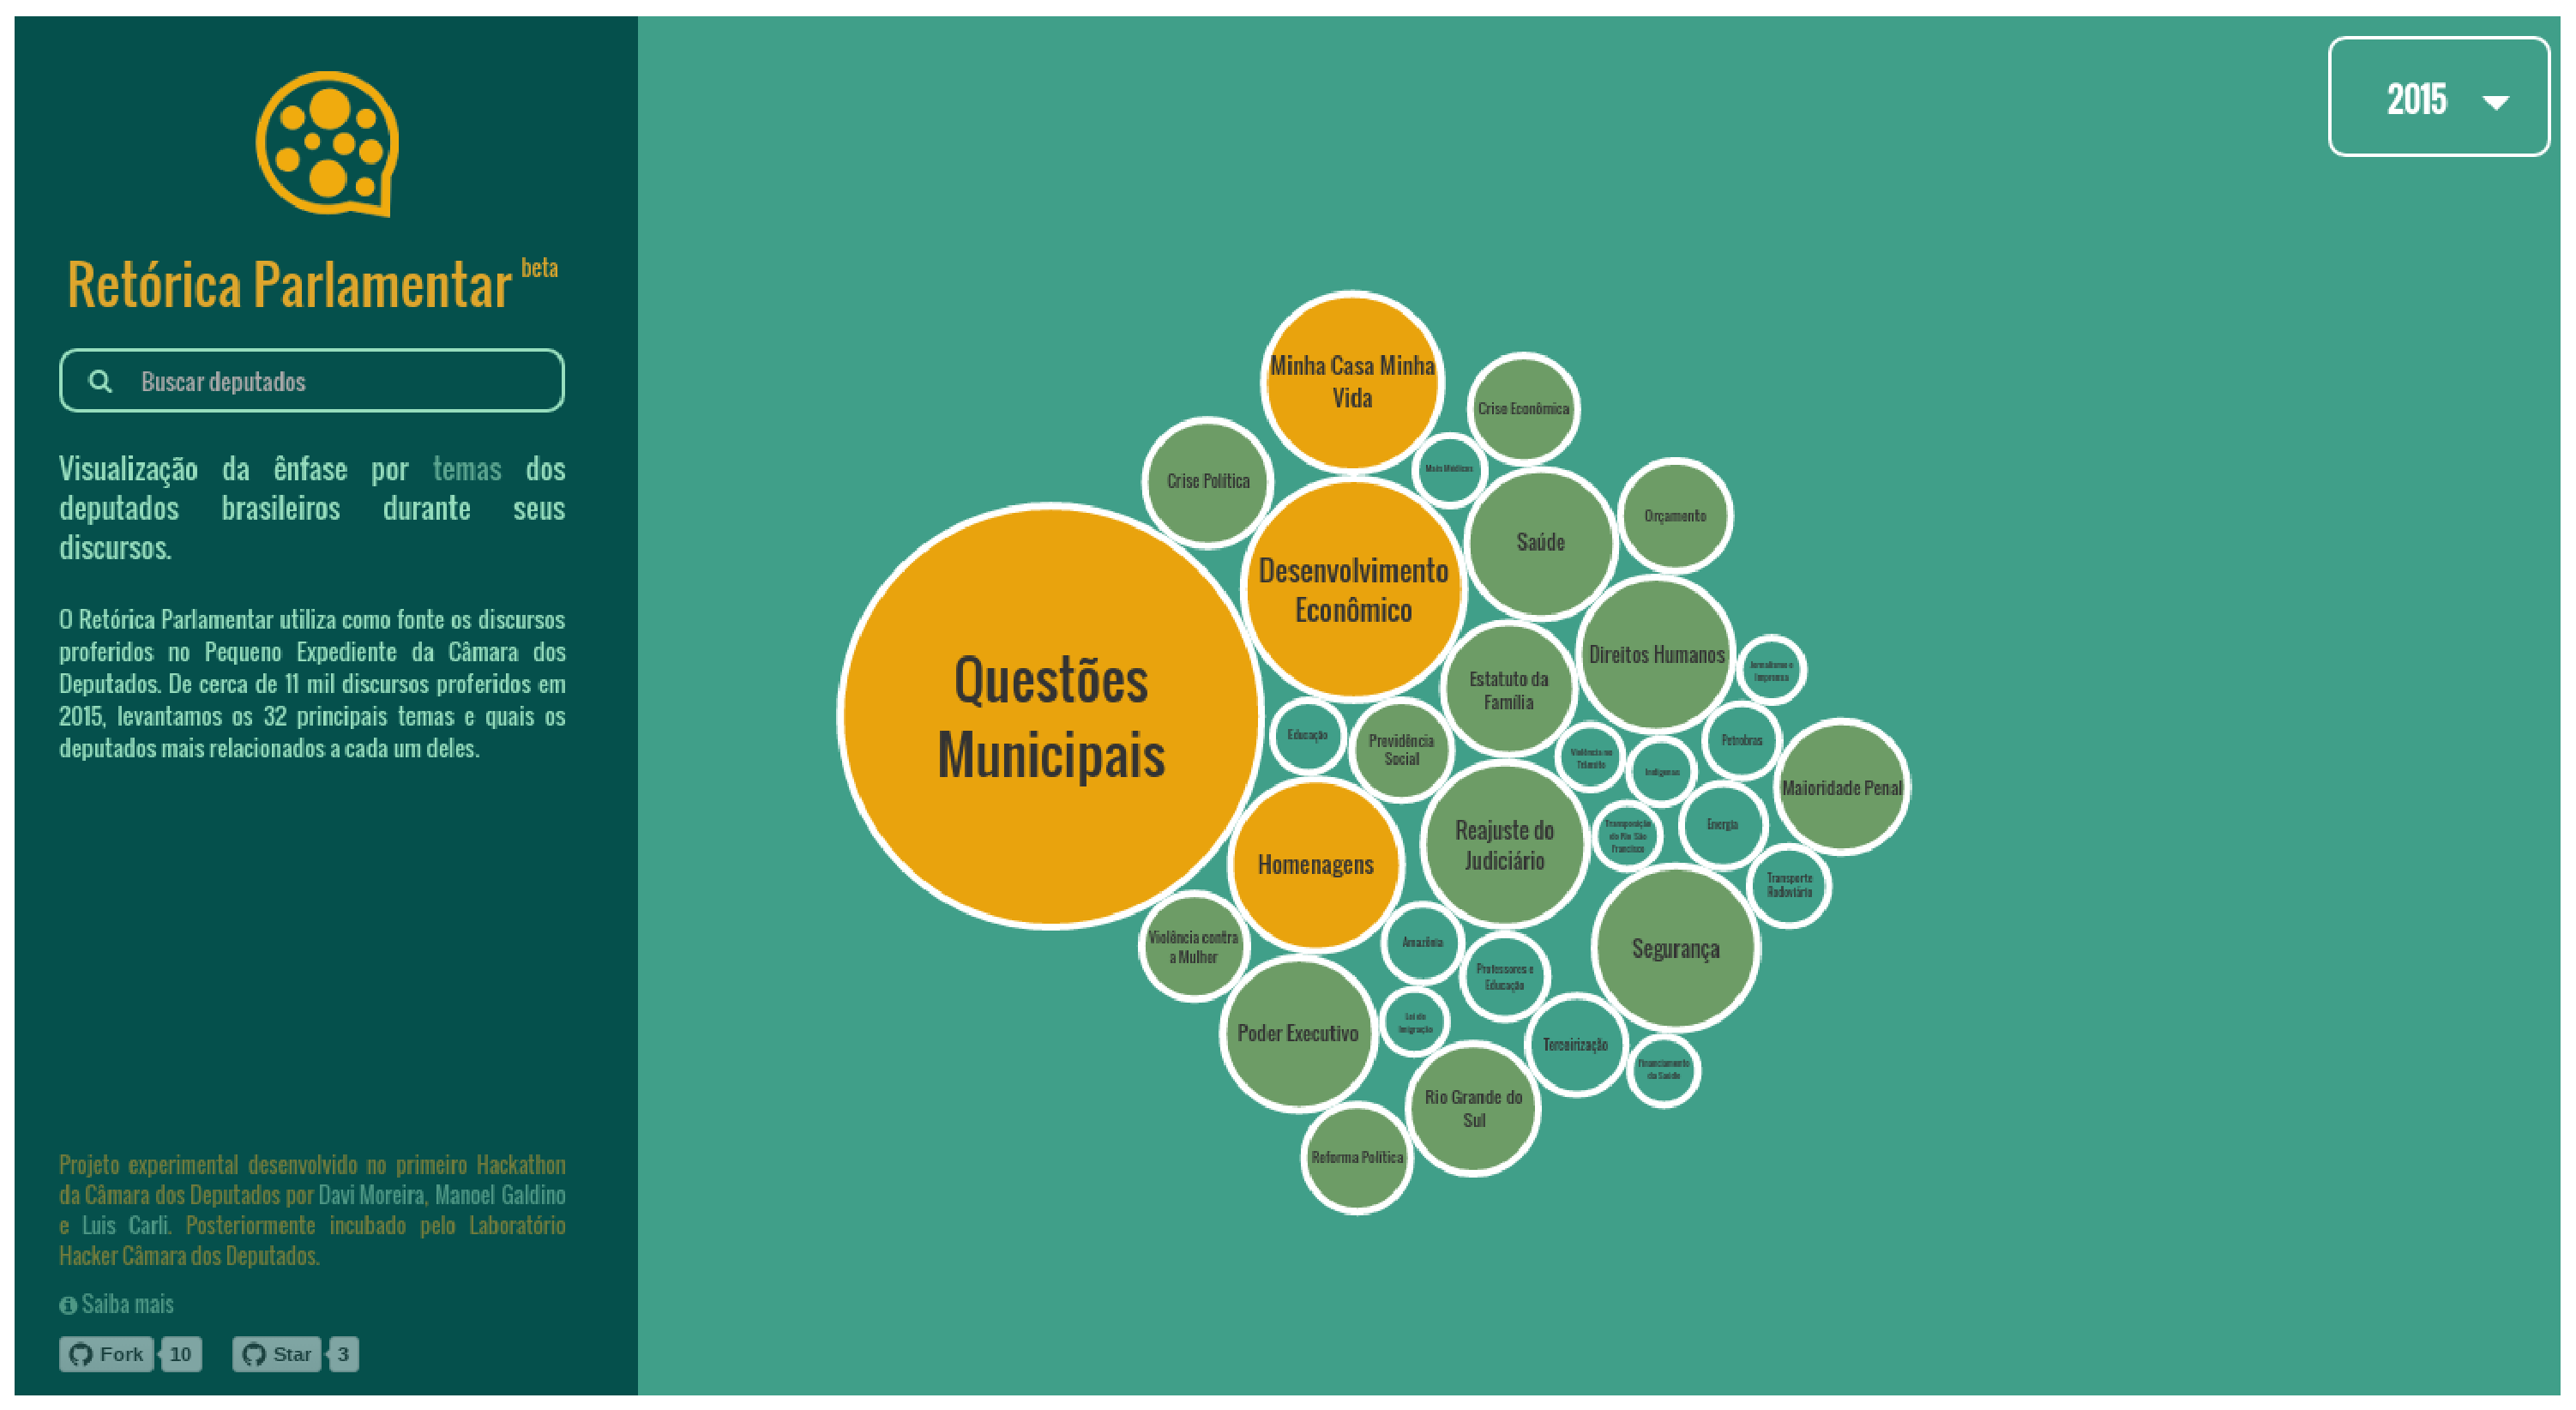
\includegraphics[scale=0.3]{figuras/retorica.eps}
    \caption{Retórica Parlamentar}
\end{figure}


\subsection{\textit{Automatic content analysis of legislative documents by text mining techniques}}

Outro trabalho encontrado foi o de \citeonline{lin}, onde propõem uma análise automática dos dados do parlamento de Taiwan, como questionamentos legislativos, discursos em conferências, proposições legislativas e proposições provisórias do Legislativo de Yuan (poder legislativo unicameral da República da China), utilizando técnicas de processamento de linguagem natural, com o objetivo de representar o desempenho de cada legislador em determinadas categorias, definidas por especialistas do \textit{Institute of Political Science} da \textit{National Sun Yat-sen University}.

\citeonline{lin} definem três aspectos para a análise dos dados do parlamento de Taiwan: direção geográfica, público-alvo e tópico. A direção geográfica se refere ao escopo geográfico abrangido pelos registros legislativos e tem 5 direções. O público-alvo refere-se às pessoas mencionadas explicitamente em seus registros, podendo ser 30 opções. O tópico inclui os temas abordados pelos parlamentares, que possuem um total de 29 tópicos. A figura abaixo mostra os três aspectos e seus valores correspondentes:

\clearpage

\begin{figure}[h]
    \centering
    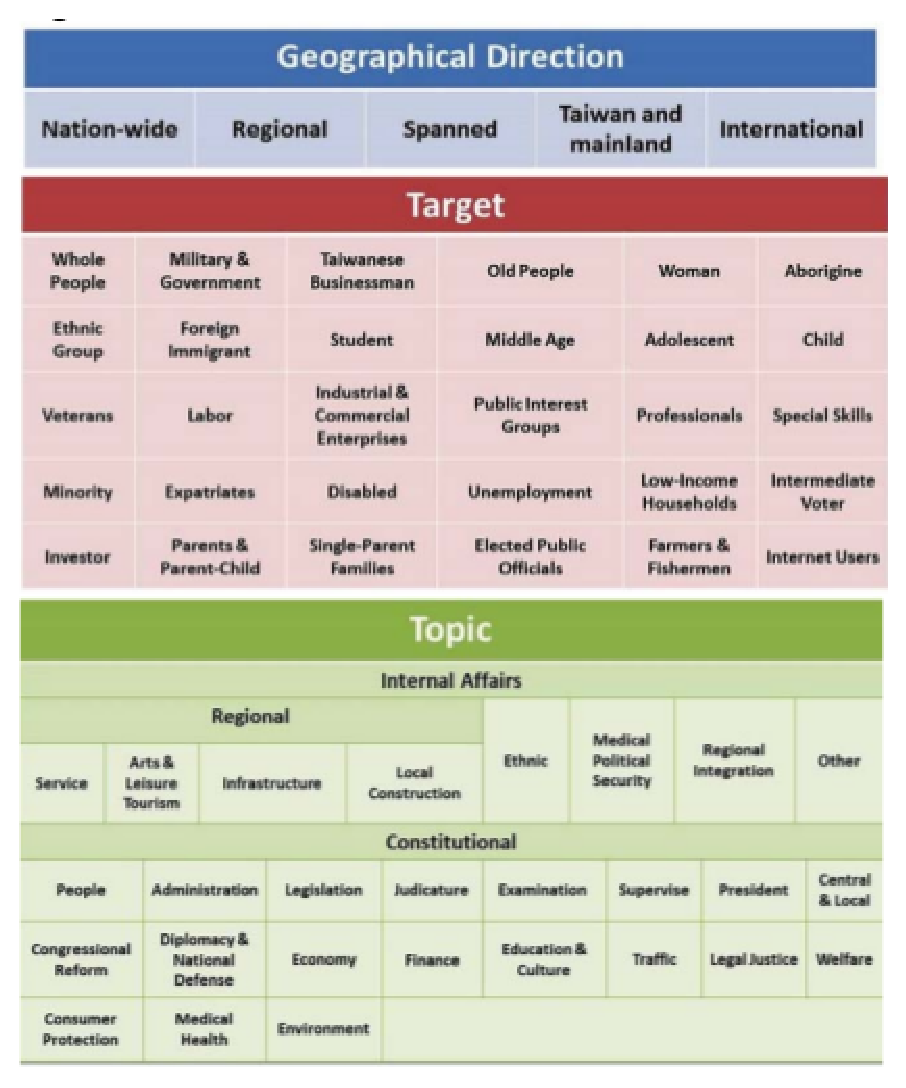
\includegraphics[scale=0.5]{figuras/aspects.eps}
    \caption{Estrutura de categorização}
\end{figure}


Após o processo de pré-processamento do texto, os dados passam por duas fases de clusterização. A primeira fase consiste em uma classificação hierárquica, com o objetivo de obter o número de \textit{clusters} ideal. Em seguida, é aplicado o \textit{k-means}, utilizando o número obtido no processo anterior como valor de \(k\). Dessa forma conseguem melhorar a relevância dos termos que serão apresentados aos especialistas para a definição dos termos que representam as classes.

Os autores disponibilizaram uma interface \textit{web} para os especialistas, para que eles classificassem os quatro tipos de texto (questionamentos legislativos, discursos em conferências, proposições legislativas e proposições provisórias). Esses textos classificados serviram como dados de treinamento e teste do modelo \textit{Support Vector Machine}, adotado para fazer a classificação.

Para representar os dados da análise, foram utilizados gráficos de radar para cada aspecto mencionado anteriormente, como mostram as figuras:

\begin{figure}[h]
  \centering
  \begin{subfigure}{.3\textwidth}
    \centering
    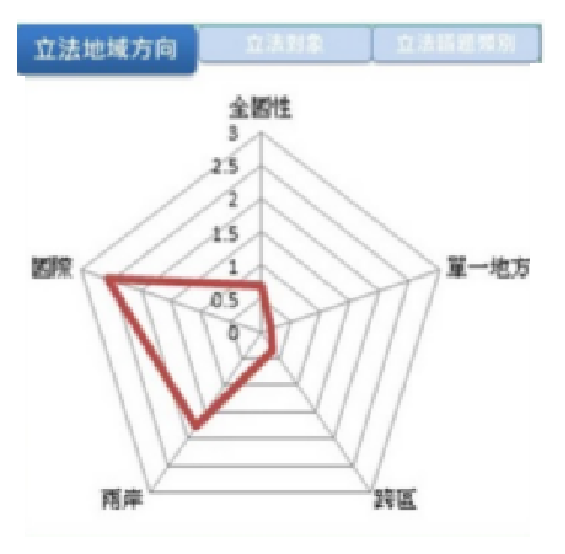
\includegraphics[scale=0.35]{figuras/aspecto1.eps}
  \end{subfigure}%
  \begin{subfigure}{.3\textwidth}
    \centering
    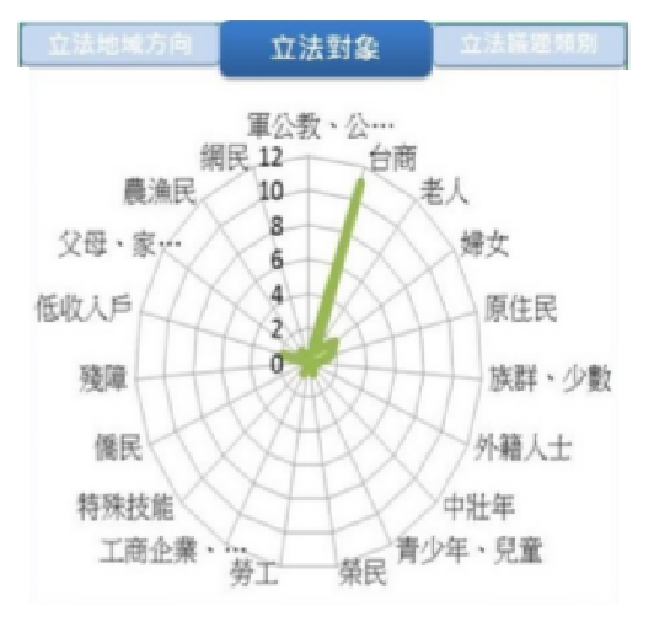
\includegraphics[scale=0.3]{figuras/aspecto2.eps}
  \end{subfigure}
  \begin{subfigure}{.3\textwidth}
    \centering
    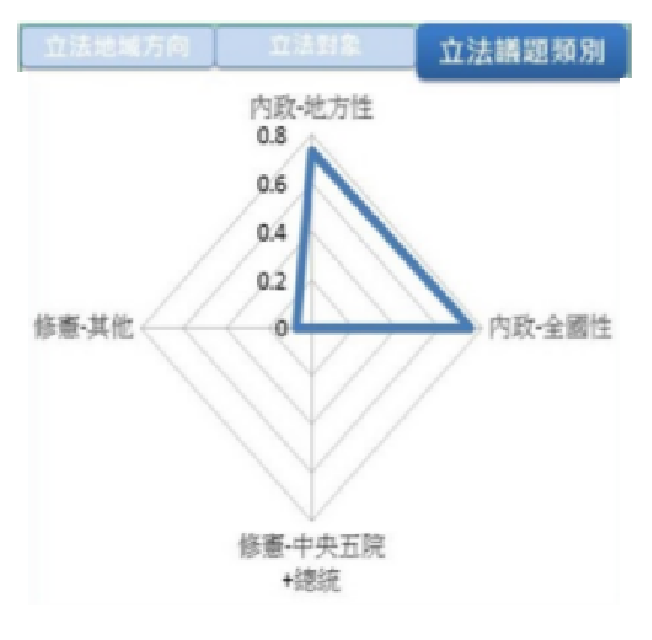
\includegraphics[scale=0.3]{figuras/aspecto3.eps}
  \end{subfigure}
  \caption{Gráficos de desempenho do parlamentar}
\end{figure}

\section{Planejamento das Atividades}

Para a realização desse trabalho, foram identificadas algumas atividades que deveriam seguir uma ordem para ser executadas, como mostra o diagrama a seguir:

\begin{figure}[h]
    \centering
    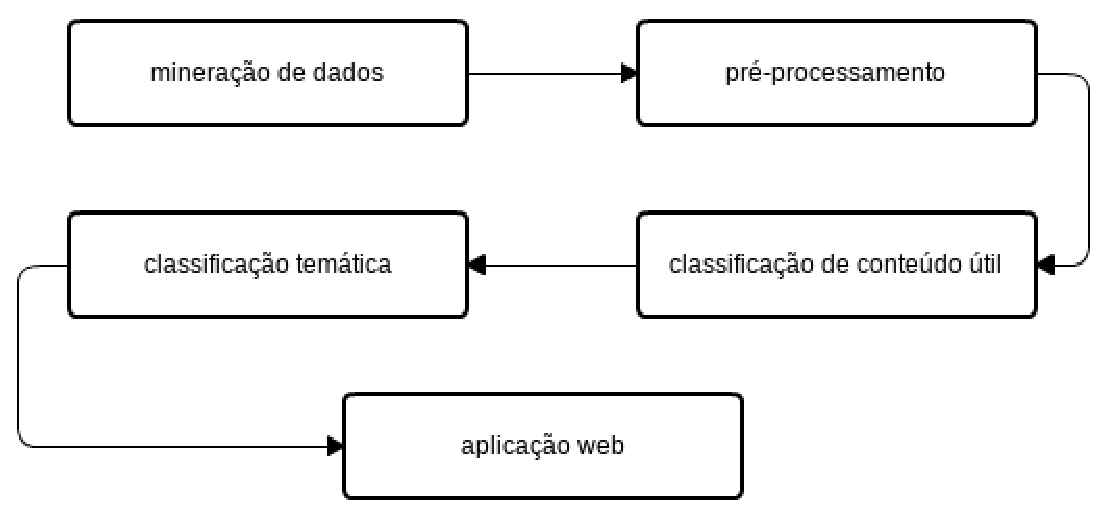
\includegraphics[scale=0.5]{figuras/planejamento.eps}
    \caption{Diagrama de planejamento}
\end{figure}

\subsection{Mineração de Dados}

A obtenção e persistência dos dados será realizada por uma biblioteca desenvolvida pelo autor, descrita na seção \ref{obtencao-dados}.

A obtenção dos dados consiste em realizar consultas ao \textit{webservice} da Câmara dos Deputados, fazendo um processamento inicial, afim de padronizar as informações e transformá-las em seus tipos correspondentes na linguagem \textit{python}. Os dados provenientes do \textit{webservice} estão em formato \textit{XML} e armazenam valores como \textit{strings}.

Nesta etapa transformamos todos os campos com valores de números inteiros e decimais, datas, horários e textos em, respectivamente, valores dos tipos \textit{int}, \textit{float}, \textit{datetime.date}, \textit{datetime.time} e \textit{str}.

\subsection{Pré-processamento}

Apesar do ``pré-processamento'' não depender tanto dos dados reais, a definição das \textit{stop words} deve ser feita levando em consideração o conteúdo que será analisado.

A etapa de pré-processamento consiste na análise dos textos obtidos na mineração de dados, afim de identificar as \textit{stop words} presentes em textos do contexto legislativo. Além disso, deve ser realizada o processo de \textit{stemização} para reduzir a dimensionalidade das \textit{bag-of-words} geradas.

Estudamos diferentes estratégias para a utilização de \(n\)-gramas, mas por enquanto decidiu-se, por uma questão de simplicidade, limitar-se apenas ao uso de unigramas.

\subsection{Classificação Conteúdo Útil}

Essa classificação tem como objetivo melhorar a qualidade da análise temática dos deputados. Uma parte considerável dos textos não possuem valor semântico significativo, pois tratam de questões protocolares e de trâmite legislativo. Citamos um exemplo: \textit{``É preciso haver quórum de 257 Srs. Deputados para aprovação da matéria, quórum mínimo. A votação é normal. Então, acho que, quando houver uns 300 ou 320 votos, encerraremos.''}. Portanto, a classificação entre conteúdo útil/não-útil consiste em separar os parágrafos que realmente possuem valor para a análise posterior dos que não devem ser usados nestas análises.

\subsection{Classificação Temática}

Após determinar quais parágrafos serão análisados, os mesmos devem ser classificados de acordo com alguns temas. Selecionamos inicialmente: Agropecuária, Saúde, Esporte, Educação, Ciência e Tecnologia, Economia, Política, Meio Ambiente, Direitos Humanos e Segurança. Para a realização dessa tarefa, foi necessário construir um texto inicial para cada um dos temas listados, afim de fornecer um parâmetro inicial ao classificador. Os textos iniciais de cada tema têm como base textos previamente classificados em portais de notícias brasileiros e consistem em apenas uma listagem de palavras comuns relacionadas a estes temas.

\subsection{Aplicação \textit{Web}}

Os dados obtidos da classificação temática serão utilizados para alimentar um sistema \textit{web} para a exibição dos
mesmos. As principais funcionalidades planejadas são: visualizar os temas mais abordados por deputados, organizados por região, partido e bancada, visualizar todos os temas de uma determinada categoria, bem como o quanto cada tema é discutido e visualizar todos os temas abordados por um determinado deputado, mostrando separadamente os temas abordados em seus discursos e nas suas proposições.

Esta parte do projeto está em fase inicial e não iniciou o desenvolvimento propriamente dito. As funcionalidades planejadas e protótipos iniciais estão disponíveis no apêndice \ref{prototipos-apendice}.

\section{Ferramentas e Tecnologias}
\label{ferramentas}

Para auxiliar no desenvolvimento, foram escolhidas as seguintes tecnologias:

\subsection{Linguagem de Programação}

Devido ao tamanho da comunidade, grande utilização na área de aprendizado de máquina, possibilidade de desenvolvimento \textit{web} e conhecimento prévio do autor e orientador, decidiu-se utilizar a linguagem \textit{Python}\footnote{https://www.python.org} para o desenvolvimento das aplicações do presente trabalho.


\subsection{\textit{Frameworks} e Bibliotecas}

O desenvolvimento da aplicação \textit{web}, utilizará o \textit{framework} \textit{Django}\footnote{https://www.djangoproject.com}, o que implica na uso da arquitetura \textit{MVT} (\textit{Model View Template}). Similar ao \textit{MVC}, no \textit{MVT} o ciclo começa por uma ação do usuário, a View notifica a Model, para que seu estado seja atualizado, a Model efetua as modificações necessárias e alerta as suas dependências que foi alterada, assim a Template consulta o novo estado da Model, e atualiza a sua visualização.

Para trabalhar com o processamento de linguagem natural e aprendizado de máquina aplicado, serão utilizadas as bibliotecas \textit{plagiarism}\footnote{https://github.com/fabiommendes/plagiarism} e \textit{texblob}\footnote{https://textblob.readthedocs.io}, que encapsula a biblioteca \textit{NLTK}\footnote{http://www.nltk.org}. Alguns cálculos são implementados utilizando o \textit{stack} científico do \textit{Python}, que inclui o \textit{numpy}\footnote{http://www.numpy.org}, \textit{scipy}\footnote{https://www.scipy.org}, \textit{matplotlib}\footnote{http://matplotlib.org} e \textit{sklearn}\footnote{http://scikit-learn.org}.


\subsection{Gerenciador de Repositórios de Código}

O gerenciamento de versões dos códigos das aplicações desenvolvidas utiliza o \textit{Git}\footnote{https://git-scm.com} e o serviço de \textit{web hosting} compartilhado \textit{GitHub}\footnote{https://github.com}. Além disso, os pacotes \textit{Python} são enviados para o \textit{PyPI}\footnote{https://pypi.python.org/pypi}, sendo facilmente instaláveis através do comando \textit{pip}\footnote{https://pip.pypa.io}.


\subsection{Documentação do Projeto}

A documentação do projeto, realizada utilizando a biblioteca \textit{Python sphinx}\footnote{http://www.sphinx-doc.org}, que possibilita a extração de documentação por meio de \textit{docstrings} no código e arquivos \textit{.rst}, e o próprio \textit{GitHub}, através de \textit{readmes} no repositório.

\subsection{Gerenciamento de Tarefas}

O controle de tarefas executadas ou em execução é feito utilizando o sistema de \textit{issues} e quadro de projetos do \textit{GitHub}.



